\section{Main elements and workflow}

Each Lambert's problem solver makes use of its own mathematical background to
approach the solution to the problem. However, all algorithms share a common
workflow in which a particular set of elements can be identified. Among these
elements it is possible to find the free-parameter, the numerical method, an
initial-guess and the velocity vectors construction procedure.

\vspace{0.5cm}
\begin{figure}[h]
  \centering
  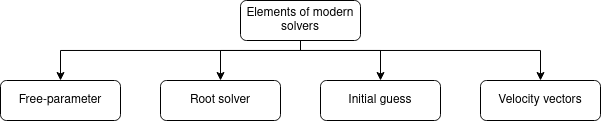
\includegraphics[width=\linewidth]{static/solver_elements.png}
  \caption{Main elements forming the basic structure of any modern Lambert's
  problem solver.}
   \label{fig:solver_elements}
\end{figure}


In the following subsections, each one of previous cited elements is explained
in detail.

\subsection{The free-parameter}

The free-parameter is the independent variable, also named the iteration
parameter. Any algorithm will reach a given equation in which this parameter is
in implicit form, meaning that a numerical method is required to obtain its
value.

Among history, several algorithms have been developed exploiting different
free-parameters such us the semi-major axis $a$, the orbit's eccentricity $e$,
the orbital parameter or semi-latus rectum $p$, the true anomaly $\nu$, the
universal formulation and finally the Kustaanheimo-Stiefel formulation.

\vspace{0.5cm}
\begin{figure}[h]
  \centering
  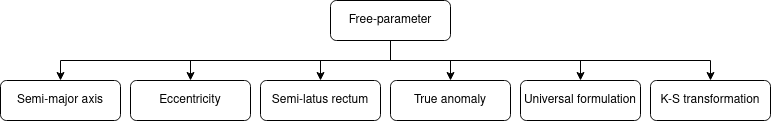
\includegraphics[width=\linewidth]{static/free_parameter.png}
  \caption{All possible free-parameters employed for solving the Lambert's problem.}
  \label{fig:free_parameter}
\end{figure}


\subsection{The numerical method}

The previously presented free-parameter is solved by means of a numerical method
or root finder. Numerical methods for solving root equations are abundant in the
literature, being some of the most common ones bisection, regula-falsi, secant,
Newton's method, Halley's method and Householder's one.

\vspace{0.5cm}
\begin{figure}[h]
  \centering
  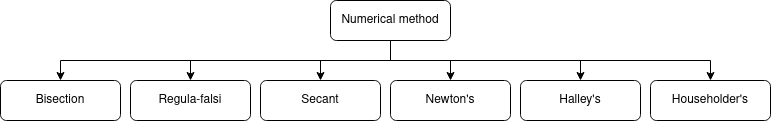
\includegraphics[width=\linewidth]{static/numerical_method.png}
  \caption{Different root finders found in literature to solve for the
  free-parameter equation.}
  \label{fig:numerical_method}
\end{figure}


The last three of the listed methods are the most common ones employed by
authors in modern solvers. However, bisection method is also employed when the
solution is known to be in a stiff region when these methods diverge, as it
always converges to the solution if the proper interval is given.

The numerical method used is strongly related with the mathematical approach
employed. Depending on the nature of the equation for the free-parameter, a
numerical method will perform better or worst than others.

Finally, it might be possible that some algorithms apply a different root finder
solver depending on the type of the orbit.

\subsection{The initial guess}

Any numerical methods always requires from an initial guess. This is the initial
value imposed to the free-parameter to start the iteration and check if its
equation fulfills.

Classic algorithms, all of those previous to the modern ones, made use of an
arbitrary initial guess without developing any additional procedure. This is no
longer the case with modern ones in which a more complex sub-routine is
developed in order to have a reliable initial guess to reduce the computation
time and achieve faster the solution.

The initial guess is dependent on the numerical method employed and thus, on the
mathematical background too. As opposite to the free-parameter or the numerical
method, there is no such a clear classification for this element. However, below
these lines, some procedures found in literature are listed: arbitrary, time of
flight for a parabolic orbit\footnote{Enables to quickly identify the shape of
the orbit by comparing the current observed one with the parabolic one.
If higher or lower, either elliptic or hyperbolic is the resultant type of
orbit.}, linear approximation and bi-linear one.

\vspace{0.5cm}
\begin{figure}[h]
  \centering
  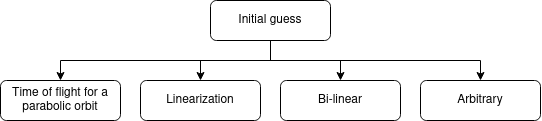
\includegraphics[width=\linewidth]{static/initial_guess.png}
  \caption{Possible approaches to be used in the initial guess procedure.}
  \label{fig:initial_guess}
\end{figure}

It must be pointed that the level of complexity of initial guess procedure
should must not be detrimental to the total computation time. Otherwise, it is
absurd to waste such a valuable time instead of letting the root solver to
perform the iteration workload.

\subsection{The velocity vectors construction}

The last sub-routine employed by any Lambert's solver is the computation of the
velocity vectors. One might thought that the computation of COE elements is also
valid but, since we are given as initial input two position vectors, it is
reasonable that the user expects the velocity ones as output so the RV is
completely defined.

There are different approaches followed by modern solvers to compute the value
of these vectors once the free-parameter has been solved such us using the
radial and tangential components, $f$ and $g$ formulation or applying a COE to
RV conversion.

\vspace{0.5cm}
\begin{figure}[h]
  \centering
  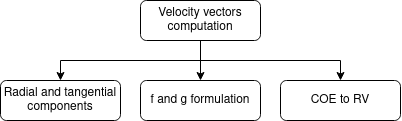
\includegraphics[scale=0.75]{static/velocity_vectors.png}
  \caption{Possible ways of constructing the initial and final velocity vectors.}
  \label{fig:velocity_vectors}
\end{figure}

